\documentclass[11pt, a4paper]{article}

% =============================================================================
% HUNARMAND — Hackathon Pitch Document
% =============================================================================

% ── Packages ─────────────────────────────────────────────────────────────────
\usepackage[margin=2.2cm, top=2.4cm, bottom=2.4cm]{geometry}
\usepackage[T1]{fontenc}
\usepackage[utf8]{inputenc}
\usepackage{lmodern}
\usepackage[expansion=false]{microtype}
\usepackage{parskip}
\usepackage{titlesec}
\usepackage{enumitem}
\usepackage{booktabs}
\usepackage{tabularx}
\usepackage{array}
\usepackage{xcolor}
\usepackage{graphicx}
\usepackage{hyperref}
\usepackage{fancyhdr}
\usepackage{multicol}
\usepackage{tcolorbox}
\usepackage{amsmath}
\usepackage{setspace}
\usepackage{tikz}
\usetikzlibrary{shapes.geometric, arrows.meta, positioning, calc, fit, backgrounds}

% ── Color Palette (Kashmir-rooted) ───────────────────────────────────────────
\definecolor{ink}{HTML}{1A1A1A}
\definecolor{lapis}{HTML}{1E3A5F}
\definecolor{saffron}{HTML}{C7811C}
\definecolor{walnut}{HTML}{5B3A1E}
\definecolor{paper}{HTML}{FAF6EC}
\definecolor{paperdark}{HTML}{EFE6D2}
\definecolor{muted}{HTML}{6B7280}
\definecolor{accent}{HTML}{B91C1C}
\definecolor{success}{HTML}{15803D}
\definecolor{rule}{HTML}{C7811C}

% ── Hyperref ─────────────────────────────────────────────────────────────────
\hypersetup{
  colorlinks=true,
  linkcolor=lapis,
  urlcolor=saffron,
  citecolor=lapis,
  pdfauthor={Team Hunarmand},
  pdftitle={Hunarmand — The Tacit Knowledge OS for Heritage Artisans},
}

% ── Typography ───────────────────────────────────────────────────────────────
\titleformat{\section}
  {\Large\bfseries\color{lapis}}
  {\thesection.}{0.6em}{}
  [\vspace{-0.25em}\color{rule}\rule{\linewidth}{1.4pt}]

\titleformat{\subsection}
  {\normalsize\bfseries\color{walnut}}
  {\thesubsection}{0.5em}{}

\titleformat{\subsubsection}
  {\normalsize\itshape\color{muted}}
  {}{0em}{}

\titlespacing{\section}{0pt}{1.5em}{0.55em}
\titlespacing{\subsection}{0pt}{0.9em}{0.3em}

% ── Header / Footer ──────────────────────────────────────────────────────────
\pagestyle{fancy}
\fancyhf{}
\fancyhead[L]{\small\textbf{\color{lapis}HUNARMAND} \color{muted}— Tacit Knowledge OS for Heritage Artisans}
\fancyhead[R]{\small\color{muted}Hackathon Pitch · 2025}
\fancyfoot[C]{\small\color{muted}\thepage}
\renewcommand{\headrulewidth}{0.4pt}
\renewcommand{\footrulewidth}{0pt}

% ── tcolorbox ────────────────────────────────────────────────────────────────
\tcbuselibrary{skins, breakable}

\newtcolorbox{heroquote}{
  colback=paper, colframe=saffron,
  left=14pt, right=14pt, top=10pt, bottom=10pt,
  arc=2pt, boxrule=1pt, breakable
}

\newtcolorbox{kashmirbox}[1][]{
  colback=paper, colframe=walnut,
  fonttitle=\bfseries\small\color{paper},
  coltitle=paper, colbacktitle=walnut,
  title=#1, attach boxed title to top left={xshift=8pt, yshift=-2pt},
  boxed title style={arc=1pt, boxrule=0pt},
  left=10pt, right=10pt, top=12pt, bottom=8pt,
  arc=2pt, boxrule=0.6pt, breakable
}

\newtcolorbox{insightbox}[1][]{
  colback=paperdark, colframe=lapis,
  fonttitle=\bfseries\small\color{paper},
  coltitle=paper, colbacktitle=lapis,
  title=#1, attach boxed title to top left={xshift=8pt, yshift=-2pt},
  boxed title style={arc=1pt, boxrule=0pt},
  left=10pt, right=10pt, top=12pt, bottom=8pt,
  arc=2pt, boxrule=0.6pt, breakable
}

\newtcolorbox{warnbox}{
  colback=red!4!white, colframe=accent,
  left=10pt, right=10pt, top=8pt, bottom=8pt,
  arc=2pt, breakable
}

\newtcolorbox{statbox}{
  colback=lapis, coltext=paper, colframe=lapis,
  left=12pt, right=12pt, top=10pt, bottom=10pt,
  arc=3pt, breakable
}

\newtcolorbox{uspbox}{
  enhanced, colback=ink, coltext=paper, colframe=saffron,
  borderline west={3pt}{0pt}{saffron},
  left=14pt, right=14pt, top=12pt, bottom=12pt,
  arc=2pt, boxrule=0pt, breakable
}

\newtcolorbox{layerbox}[1][]{
  enhanced, colback=paper, colframe=lapis,
  fonttitle=\bfseries\color{paper},
  coltitle=paper, colbacktitle=lapis,
  title=#1, attach boxed title to top left={xshift=8pt, yshift=-2pt},
  boxed title style={arc=2pt, boxrule=0pt},
  left=12pt, right=12pt, top=14pt, bottom=10pt,
  arc=3pt, boxrule=0.8pt, breakable
}

% ── Lists ────────────────────────────────────────────────────────────────────
\setlist[itemize]{leftmargin=1.3em, itemsep=2pt, topsep=3pt}
\setlist[enumerate]{leftmargin=1.4em, itemsep=2pt, topsep=3pt}

% =============================================================================
\begin{document}
% =============================================================================

% ── Title block ──────────────────────────────────────────────────────────────
\begin{center}
  {\fontsize{42}{46}\selectfont\bfseries\color{lapis} HUNARMAND}\\[2pt]
  {\small\color{saffron}\itshape\textbf{hunar-mand}\,\textbar\,Persian-Urdu-Kashmiri\,\textbar\,(noun) the skilled one; one who carries craft inside them}\\[12pt]
  {\Large\color{walnut}\itshape The Tacit Knowledge OS for Heritage Artisans}\\[10pt]
  {\small\color{muted} Hackathon Pitch · NIT Srinagar · Team of 5 · 2025}
\end{center}

\vspace{0.4em}
\noindent\color{rule}\rule{\linewidth}{1.5pt}
\vspace{0.6em}

% ── Hero quote ───────────────────────────────────────────────────────────────
\begin{heroquote}
\centering
\itshape\large\color{walnut}
``A 70-year-old Pashmina master in Kanihama does not just know how to weave. \\[3pt]
He knows which wool from which Ladakh village has the right micron count. \\[3pt]
Why warp tension changes in winter humidity. The dye ratios his grandfather \\[3pt]
developed that no book has ever recorded. When he passes, all of it goes with him. \\[6pt]
\bfseries\color{saffron} That is the same problem big companies face when their senior \\[3pt]
engineers quit --- just ten times more irreversible.''
\end{heroquote}

% =============================================================================
\section{The One-Sentence Pitch}
% =============================================================================

\begin{uspbox}
\textbf{Hunarmand is the Tacit Knowledge OS for heritage artisans. We capture the irreplaceable knowledge that dies with the master --- the unwritten techniques, supplier secrets, environmental tunings, and decades of failed experiments --- and turn it into a verified provenance layer that counterfeiters cannot fake, a workshop economy tourists pay a premium for, and a heritage bazaar that scales authenticity into commerce. The artisan's mind becomes their most valuable asset. The platform makes that asset finally pay them.}
\end{uspbox}

% =============================================================================
\section{The USP Nobody Else Can Copy}
% =============================================================================

\begin{insightbox}[The Reframe That Wins The Room]
Every other team in this hackathon will pitch a craft \textit{marketplace}. We are not pitching a marketplace. We are pitching {\bfseries infrastructure for a kind of knowledge no platform on earth currently protects}: the tacit, undocumented, hand-held knowledge that lives only inside a master craftsman's body and dies in the same room.\\[5pt]
The exact same problem occurs inside every large engineering organisation when senior engineers leave: critical context evaporates, no one knows why a system was built the way it was, and the next generation re-invents the broken parts. Big tech spends billions on internal Confluence pages, RFCs, and tribal-knowledge handovers to fix this. {\bfseries Kashmir's master craftsmen have nothing.} When they pass, they take centuries with them.\\[5pt]
Hunarmand is the first platform that treats artisans the way modern engineering treats institutional memory --- as a strategic, captureable, monetisable asset. Then it builds the commercial layers (directory, workshops, bazaars, direct commerce) on top of that captured knowledge so the artisan finally gets paid for what only they know.
\end{insightbox}

\subsection{Five things this framing gives us that a marketplace cannot}

\begin{enumerate}
  \item \textbf{A new category nobody owns.} ``Tacit Knowledge OS for craft'' is a phrase no incumbent has uttered. Etsy is a marketplace. INTACH is an archive. We are neither.
  \item \textbf{Counterfeit-proof provenance.} A fake shawl can be made. The 1940s knot pattern Mohammad Yusuf's grandfather invented, with the specific failure modes only this lineage knows, cannot. Captured tacit knowledge is the only authentication that scales.
  \item \textbf{Premium pricing power.} Buyers do not pay for ``handmade.'' They pay for \textit{provenance}. Hunarmand is the only place that can price provenance, because it is the only place that captured what makes it real.
  \item \textbf{An irreversible moat.} Every interview locked into the Hunarmand Vault is unrepeatable. A competitor starting later cannot interview a master who has died. The moat compounds on a biological clock.
  \item \textbf{Dignity for the artisan.} ``Marketplace seller'' is a transactional identity. ``Knowledge holder whose institutional memory is digitised, owned, and licensed'' is a generational identity. The artisan's children re-enter the craft because the craft now carries status.
\end{enumerate}

% =============================================================================
\section{The Problem, Stated Plainly}
% =============================================================================

A 72-year-old {\itshape ustaad} of {\itshape sozni} embroidery sits in a wooden workshop on the second floor of a building in Downtown Srinagar. He threads a needle that he has held since he was nine. His son drives a taxi in Sopore. His grandson is studying for an exam in Bengaluru. Neither of them can sozni a single petal.

The {\itshape ustaad} will pass away in this decade. With him will go a stitch no museum has, no book has captured, no algorithm has ever seen. Multiply that by the master {\itshape Kani} weaver in Kanihama, the {\itshape khatamband} ceiling-maker in Zaina Kadal, the {\itshape naqash} who layers gold on papier-m\^{a}ch\'{e} in Rainawari. Multiply by ten thousand workshops. This is what is happening in Kashmir, right now, this season.

\begin{statbox}
\textbf{The four facts that frame this hackathon:}\\[4pt]
\textbf{1.} Kashmir's craft sector employs \textbf{\textasciitilde 4 lakh artisans} and exports \textbf{\textasciitilde Rs.\ 1{,}600 crore} annually --- yet over \textbf{60\%} of ``Kashmiri'' goods sold globally are counterfeits made elsewhere.\\[3pt]
\textbf{2.} The average age of a Kashmiri master craftsman has risen from 36 (1980s) to over \textbf{55 today}. New apprentice enrolment in traditional crafts has fallen by \textbf{more than 50\%} in two decades.\\[3pt]
\textbf{3.} Children of master artisans cite three reasons for not entering the craft: \textbf{(a)} middlemen take \textbf{70--85\%} of end-buyer value, \textbf{(b)} the family name never reaches the buyer, \textbf{(c)} no inheritable asset --- when the master passes, nothing systematic is left behind.\\[3pt]
\textbf{4.} Less than \textbf{1\%} of Kashmiri craft businesses have any structured documentation of their own techniques, suppliers, or pricing logic. This is the same risk profile a company with no documented systems carries when a key engineer quits --- except here, the engineer is dying.
\end{statbox}

\subsection{Why existing platforms cannot solve this}

\begin{center}
\small
\begin{tabularx}{\linewidth}{>{\bfseries}lXX}
\toprule
Platform & What it does & Why it fails the artisan \\
\midrule
Etsy / Amazon Handmade & Sells handmade goods globally & No verification; floods of counterfeits; nothing about the artisan is captured beyond a profile photo \\
GI Tag (Kashmir Pashmina, etc.) & Legal protection of category names & Protects the {\itshape category}, not individual masters or their specific techniques; no record survives the artisan \\
Instagram / YouTube & Free social and content platform & The account dies with the artisan; no structure; no provenance; no commerce trust \\
Museum / INTACH archives & Preserve historical objects & One-way, passive, not connected to the artisan's commerce or income \\
Govt.\ skill schemes (PMKVY etc.) & Train new artisans on generic curricula & Bypass the master entirely; do not capture anything from existing masters \\
\bottomrule
\end{tabularx}
\end{center}

None of these capture the tacit layer. None of them route trust into income. None of them survive the master's death. Hunarmand does all three.

% =============================================================================
\section{The Solution: Hunarmand's Four Layers}
% =============================================================================

We deliberately reduced Hunarmand to \textbf{four interlocking layers}, each one feeding the next. Layer~1 produces the asset. Layers~2--4 monetise it. Together they form the flywheel that pulls a young Kashmiri back into the workshop.

\begin{center}
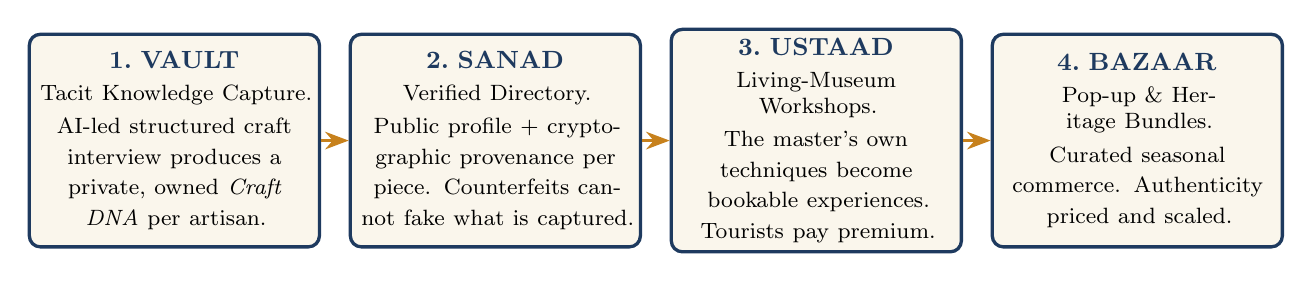
\begin{tikzpicture}[
    node distance=1.0cm and 0.35cm,
    pillar/.style={rectangle, rounded corners=4pt, draw=lapis, very thick, fill=paper, text width=3.45cm, minimum height=2.7cm, align=center, font=\small},
    flowarrow/.style={-{Stealth[length=3mm]}, thick, color=saffron},
  ]
  \node[pillar] (vault) {\textbf{\color{lapis}1.\ VAULT}\\[2pt]
    \footnotesize Tacit Knowledge Capture.\\[1pt]
    AI-led structured craft interview produces a private, owned \textit{Craft DNA} per artisan.};
  \node[pillar, right=of vault] (sanad) {\textbf{\color{lapis}2.\ SANAD}\\[2pt]
    \footnotesize Verified Directory.\\[1pt]
    Public profile + cryptographic provenance per piece. Counterfeits cannot fake what is captured.};
  \node[pillar, right=of sanad] (ustaad) {\textbf{\color{lapis}3.\ USTAAD}\\[2pt]
    \footnotesize Living-Museum Workshops.\\[1pt]
    The master's own techniques become bookable experiences. Tourists pay premium.};
  \node[pillar, right=of ustaad] (bazaar) {\textbf{\color{lapis}4.\ BAZAAR}\\[2pt]
    \footnotesize Pop-up \& Heritage Bundles.\\[1pt]
    Curated seasonal commerce. Authenticity priced and scaled.};

  \draw[flowarrow] (vault.east) -- (sanad.west);
  \draw[flowarrow] (sanad.east) -- (ustaad.west);
  \draw[flowarrow] (ustaad.east) -- (bazaar.west);
\end{tikzpicture}
\end{center}

% --- Layer 1 ---------------------------------------------------------------
\begin{layerbox}[Layer 1 \;\textbar\; VAULT --- The Tacit Knowledge Capture Engine]

\textbf{Purpose:} Take everything inside a master's head and put it into a permanent, structured, queryable, artisan-owned record --- in their own voice, in Koshur, in a single sitting they can complete on a basic phone.

\textbf{The session} runs as four guided passes by an AI interviewer trained on Kashmiri craft terminology. A field facilitator (an NIT Srinagar volunteer, a CDI student, or a family member) holds the phone:

\begin{itemize}
  \item \textbf{Pass 1 --- Lineage \& Identity.} Generation in practice. Master who taught them. Village. Family workshop history.
  \item \textbf{Pass 2 --- Technique walkthrough.} Phone is mounted; the master performs and narrates one full technique. AI probes for tool names, thread counts, hand positions.
  \item \textbf{Pass 3 --- The decision questions.} The most valuable pass. {\itshape ``How do you know the wool is good? What changes you make in winter humidity? Which mistake did your teacher correct most often? Which suppliers will copy you and which will not?''} This is the layer no apprentice ever asks and no archive has ever captured.
  \item \textbf{Pass 4 --- Material \& supplier graph.} Where wool, dye, wood, mineral pigments come from. Which villages, seasons, suppliers. Their family's specific dye ratios and natural-fibre tests.
\end{itemize}

\textbf{The output --- the Craft DNA file --- contains:}

\begin{itemize}
  \item Master's biography, lineage chain, and verification metadata
  \item Indexed video segments by named technique and tool
  \item Transcribed and translated voice in Koshur, Urdu, English (and on demand: French, Japanese, German for export buyers)
  \item A \textbf{technique knowledge graph}: techniques $\to$ sub-steps $\to$ tools $\to$ materials $\to$ environmental tunings $\to$ failure modes
  \item A \textbf{supplier provenance graph}: which materials, which villages, which seasons, which trusted suppliers
  \item A \textbf{cryptographic identity} (Ed25519 keypair) so the artisan can sign authenticity certificates on physical pieces
\end{itemize}

\textbf{The artisan owns this file.} It is private by default. They choose what becomes public on their Sanad profile. They can export it, license it to researchers, will it to their family, or take it off the platform. We are not a record; we are a vault.

\textbf{Why ``Tacit OS'' is technically correct, not marketing.} What we capture is not just data --- it is the {\itshape why} behind every decision. A photograph captures the shawl. A standard intake form captures the bio. We capture the master's reasoning, the warnings he would give, the quiet rules he follows without thinking. That is what Polanyi called {\itshape tacit knowledge}, and that is what every system has failed to capture until now.
\end{layerbox}

% --- Layer 2 ---------------------------------------------------------------
\begin{layerbox}[Layer 2 \;\textbar\; SANAD --- The Verified Directory \& Provenance Layer]

\textbf{Purpose:} Turn the captured Craft DNA into a public, searchable, trust-bearing directory --- and turn every authenticated piece into an unforgeable provenance chain.

\textbf{The Sanad profile.} Each artisan's public page is auto-populated from their Craft DNA (with the artisan's explicit consent on what becomes public). Instead of {\itshape ``Mohammad Yusuf --- Carpet Weaver, Srinagar''}, the buyer sees:

\begin{quote}
\itshape ``Mohammad Yusuf, 4th-generation hand-knotted carpet weaver, workshop in Khanyar. Holds a discontinued Srinagar knot pattern from 1940s. Sources Gurez Valley wool exclusively. Verified by the Kashmir Craft Council. 312 pieces signed; 0 disputes.''
\end{quote}

\textbf{The Sanad on every piece.} Every authenticated product carries a small QR code (woven, embossed, or printed depending on craft) that resolves to a public provenance page showing:

\begin{itemize}
  \item The artisan who made it, with full Sanad profile link
  \item The specific technique used, with a 30-second clip from the artisan's Vault
  \item Material origin: which village, which supplier, which season's batch
  \item A \textbf{cryptographic signature} (Ed25519) of the piece's metadata, signed by the artisan's keypair --- verifiable offline, anywhere, by any phone
  \item Endorsements from craft councils, recognised masters, or local guilds
  \item A fair-price band based on technique complexity and verified peer pricing
\end{itemize}

\textbf{Why this destroys counterfeits.} A Chinese knockoff can copy the look of a shawl. It cannot:
\begin{itemize}
  \item Forge a verifiable Ed25519 signature linked to a specific artisan
  \item Produce the captured tacit narrative the real artisan recorded in his Vault
  \item Show a documented supplier graph of Gurez Valley wool batch numbers
\end{itemize}

A buyer in Tokyo, Paris, Delhi, or on Lal Chowk scans the code and sees, in their language, exactly who made it, how, and from what. A missing or unverifiable Sanad becomes the universal counterfeit signal.

\textbf{Public discovery} --- the directory is fully searchable: by craft, by technique, by lineage, by village, by certification level. Buyers, designers, journalists, and researchers can find masters they would otherwise never know existed.
\end{layerbox}

% --- Layer 3 ---------------------------------------------------------------
\begin{layerbox}[Layer 3 \;\textbar\; USTAAD --- Living-Museum Workshop Marketplace]

\textbf{Purpose:} Convert the same captured tacit knowledge into the highest-margin commercial offering in the entire heritage economy: \textbf{the master's studio as a destination, the master's technique as the experience}.

\textbf{Why this is worth more than any product sale.} A tourist who watches a carpet being knotted for ten minutes becomes a story-teller. A tourist who knots ten rows under a verified master becomes a buyer for life. Until now, this revenue stream has been almost entirely informal and almost entirely uncaptured by artisans.

\textbf{Workshop offerings, structured around the artisan's Vault content:}

\begin{center}
\small
\begin{tabularx}{\linewidth}{>{\bfseries}lXX}
\toprule
Format & What the visitor gets & Indicative price \\
\midrule
Heritage Walk (2--3 hr) & Curated visit to 3--5 verified workshops in a craft cluster, with a guide using the Sanad map as itinerary & Rs.\ 1{,}500 -- 3{,}500 / person \\
Master Session (1--2 hr) & A private demonstration with a Sanad-verified master & Rs.\ 2{,}500 -- 8{,}000 / person \\
Half-Day Workshop & Hands-on basic technique; participant takes home their attempt + a Hunarmand certificate & Rs.\ 4{,}000 -- 8{,}000 \\
Multi-Day Masterclass & Specific advanced technique (e.g., the 1940s Srinagar knot) taught directly by the master who holds it & Rs.\ 25{,}000 -- 1{,}50{,}000 \\
Virtual Live Workshop & International audiences join via video; pre-shipped materials kit; live session with translation & Rs.\ 1{,}500 -- 5{,}000 \\
\bottomrule
\end{tabularx}
\end{center}

\textbf{The differentiator.} Tourists do not book a generic weaving class. They book {\itshape ``Learn the Gurez Valley Pashmina technique from a 4th-generation master, including the wool-selection process, the winter tension adjustment, and the original 1940s knot pattern.''} That is not a workshop --- that is a living museum experience, and it commands living-museum prices.

\textbf{Booking infrastructure.} Calendar management, capacity, materials kits, multilingual confirmations, automated payouts. Tour-operator and travel-platform integrations (Airbnb Experiences, Viator, Visit Kashmir). A 12--15\% platform fee. The artisan keeps the rest.
\end{layerbox}

% --- Layer 4 ---------------------------------------------------------------
\begin{layerbox}[Layer 4 \;\textbar\; BAZAAR --- Pop-up Bazaars \& Heritage Bundles]

\textbf{Purpose:} Scale authenticity into commerce at volume. The Vault makes everything verifiable; the Sanad makes everything trustworthy; the Bazaar moves everything at scale.

\textbf{Three commerce surfaces, all anchored by Sanad-verified profiles underneath:}

\begin{itemize}
  \item \textbf{The Hunarmand Bazaar (always-on online storefront).} Each artisan's verified directory page links straight to their commerce page. Multi-currency, multi-language, integrated international shipping with auto-generated heritage certificates and customs paperwork. Platform commission \textbf{6--9\%} --- compared to the 70--85\% the existing middleman chain extracts.

  \item \textbf{Pop-up Bazaars (seasonal physical + online events).} Curated, themed events that gather verified artisans for limited windows: {\itshape Tulip-Festival Bazaar, Winter Pashmina Bazaar, Eid \& Diwali Heritage Bazaar, Christmas Export Bazaar}. Hosted physically in Srinagar / Delhi / Mumbai and mirrored as live online events. Each pop-up creates a press cycle, an Instagram cycle, and a buying cycle around verified Kashmiri makers.

  \item \textbf{Heritage Bundles (curated multi-piece packages).} Cross-artisan, cross-craft bundles with a unifying narrative: {\itshape The Pampore Saffron \& Tea Trio} (verified saffron + walnut wood box + copperware spoon). {\itshape The Kanihama Pashmina Set.} {\itshape The 7-Day Heritage Trail} (workshops + bazaar credits + curated stays). Each bundle carries a single composite Sanad and a single QR. Premium gifting, corporate, and export segments.
\end{itemize}

\textbf{The economic transformation per artisan.} The combined Sanad premium + workshop revenue + bazaar revenue takes a typical Kashmiri master from a Rs.\ 12{,}000--20{,}000/month middleman-bound income to a realistic Rs.\ 60{,}000--1{,}20{,}000/month range. \textbf{That is the only number that brings a young Kashmiri back into the workshop.} Not a slogan, not a scheme --- that table.

\begin{center}
\small
\begin{tabularx}{\linewidth}{Xrr}
\toprule
\textbf{Piece (illustrative)} & \textbf{Artisan today} & \textbf{Artisan with Hunarmand} \\
\midrule
Sozni shawl, end retail Rs.\ 60{,}000 & Rs.\ 6{,}000 -- 9{,}000 & Rs.\ 54{,}000 -- 56{,}000 \\
Hand-knotted carpet, end retail Rs.\ 2{,}50{,}000 & Rs.\ 18{,}000 -- 35{,}000 & Rs.\ 2{,}30{,}000 -- 2{,}35{,}000 \\
Naqashi papier-m\^{a}ch\'{e} box, end retail Rs.\ 8{,}000 & Rs.\ 800 -- 1{,}200 & Rs.\ 7{,}200 -- 7{,}500 \\
Half-day workshop, 6 participants @ Rs.\ 6{,}000 & Rs.\ 0 (informal / never charged) & Rs.\ 30{,}000+ per session \\
\bottomrule
\end{tabularx}
\end{center}
\end{layerbox}

% =============================================================================
\section{The Hunarmand Flywheel}
% =============================================================================

\begin{insightbox}[Why the four layers form a single self-reinforcing system]
\textbf{Vault} captures the irreplaceable knowledge before it dies. \textbf{Sanad} converts that knowledge into verifiable trust that buyers will pay a premium for. \textbf{Ustaad} turns the same knowledge into bookable experiences that earn 5--20$\times$ the margin of a single product sale. \textbf{Bazaar} scales authenticity through curated commerce so the artisan finally has an income that justifies passing the craft to the next generation.\\[5pt]
The flywheel: \textbf{Capture $\to$ Trust $\to$ Premium $\to$ Income $\to$ Youth return $\to$ New apprentices $\to$ New masters $\to$ More capture.} Every other model in this space gets weaker over time --- because every year more masters die without being recorded. Hunarmand gets stronger over time, because every year more masters \textit{are} recorded, and each captured Vault is unrepeatable.
\end{insightbox}

% =============================================================================
\section{Hackathon Scope --- What We Will Actually Demo}
% =============================================================================

We will not demo all four layers at full fidelity. We will demo \textbf{one craft, one master, one buyer, one workshop, one bazaar entry, end-to-end}. The chosen vertical is \textbf{Pashmina (Kanihama lineage) with a secondary Sozni piece}. Pashmina because: (a) it carries the highest global brand recognition, (b) it has the worst counterfeit problem (the strongest demonstration of provenance value), (c) it photographs and demos beautifully on a phone.

\subsection{The 10-minute live demo flow}

\begin{enumerate}
  \item \textbf{[1 min] The shawl on the table.} Hand the jury a real Kashmiri shawl with a Hunarmand QR. They scan; the Sanad page loads. They see the master's name, his workshop, his lineage, a 30-second clip of him weaving, and a verified Ed25519 signature. They scan a counterfeit (no Sanad). The app responds: {\itshape ``No verified Sanad on this piece. Ask the seller.''}
  \item \textbf{[3 min] Vault walkthrough.} On screen: a recorded Vault session. AI interviewer asks the master in Koshur about his winter humidity adjustment. Master answers. Live: transcript appears in Koshur, then auto-translates to English. The Craft DNA technique graph populates in real time on the right.
  \item \textbf{[2 min] Sanad directory.} Switch to the public directory. Search {\itshape ``Pashmina, Gurez wool, 4th gen+''}. Three verified masters appear. Open one profile --- show the lineage chain, technique list, and a buyer-side ``Ask the Hunarmand'' that answers a question by quoting the master's own Vault clip.
  \item \textbf{[2 min] Ustaad workshop booking.} Show a Heritage Walk listing for that artisan's lineage. Pick a date. Add to cart. Test-payment confirms the booking; an email is sent in the buyer's language; the artisan's dashboard receives the booking instantly.
  \item \textbf{[1 min] Bazaar.} Open the seasonal pop-up Bazaar landing page. Show a Heritage Bundle (\textit{Kanihama Pashmina Set}) with a composite Sanad. One click checkout.
  \item \textbf{[1 min] Close on the flywheel.} One sentence: {\itshape ``One master. One Vault. One Sanad. One workshop. One bazaar entry. The same loop scales to ten thousand workshops.''}
\end{enumerate}

\subsection{Build-or-die hackathon deliverables}

\begin{center}
\small
\begin{tabularx}{\linewidth}{>{\bfseries}lX}
\toprule
Deliverable & What ``done'' looks like \\
\midrule
Vault — Master Studio (web) & Working AI-led interview with audio + video capture, Koshur (with Urdu fallback) transcription, English translation, structured Craft DNA JSON output \\
Vault viewer dashboard & Master can view their captured Craft DNA --- lineage, indexed clips, technique graph, supplier graph, vulnerability flags \\
Sanad directory & Public, searchable artisan profiles auto-populated from Craft DNA; Sanad-verified badge \\
Sanad provenance page & Per-piece QR-resolved page showing master, technique clip, supplier graph, and a verifiable Ed25519 signature \\
Ustaad booking & A working workshop calendar + booking form + test-payment + email confirmation \\
Bazaar storefront & A simple buy-now flow + one Heritage Bundle with a composite Sanad \\
Demo dataset & ONE real or carefully staged Pashmina master Vault session, recorded and processed before demo day \\
\bottomrule
\end{tabularx}
\end{center}

\subsection{Out of scope for the hackathon}

\begin{itemize}
  \item Native mobile apps (web is mobile-responsive; native is post-hack)
  \item Multi-master, multi-craft scaling (one master, one secondary craft, end-to-end is enough)
  \item Live integrations with Airbnb / Viator / Visit Kashmir (mocked listings only)
  \item Government / GI integration (planned partnership in deck, not coded)
\end{itemize}

% =============================================================================
\section{Technical Architecture}
% =============================================================================

\begin{center}
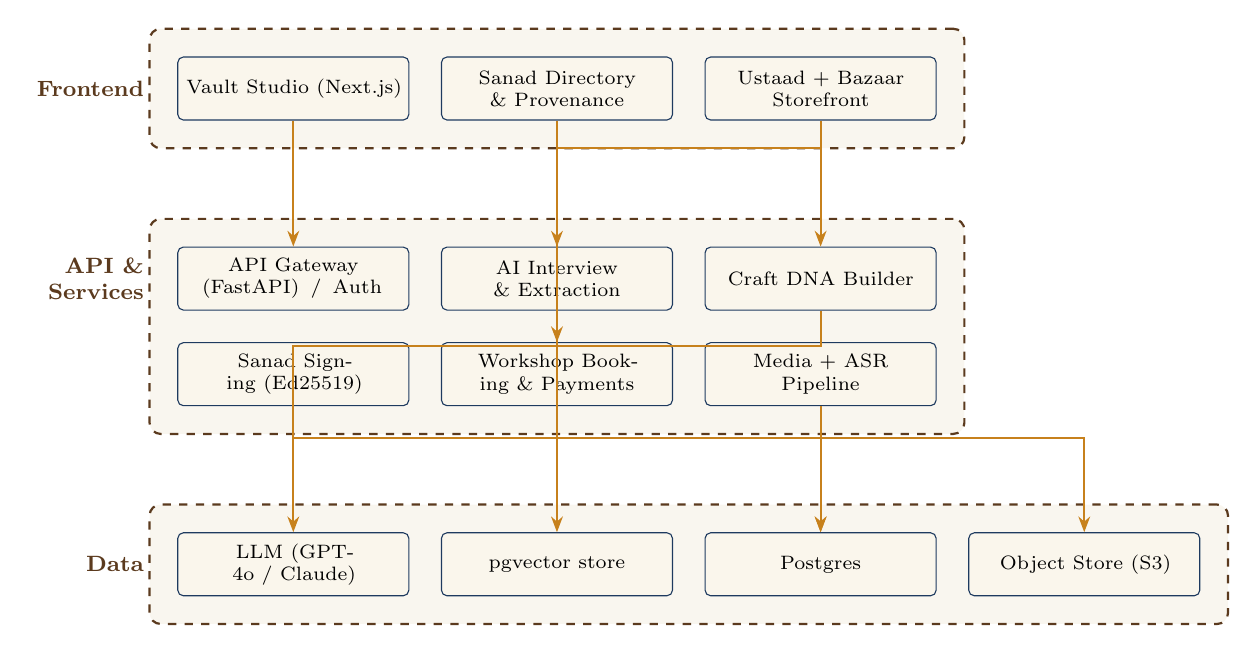
\begin{tikzpicture}[
    box/.style={rectangle, rounded corners=2pt, draw=lapis, fill=paper, text width=2.7cm, minimum height=0.8cm, align=center, font=\scriptsize},
    layerbg/.style={rectangle, rounded corners=4pt, draw=walnut, dashed, thick, fill=paperdark, fill opacity=0.35, inner sep=10pt},
    layerlabel/.style={font=\bfseries\footnotesize\color{walnut}, align=right},
    arr/.style={-{Stealth[length=2mm]}, thick, color=saffron},
  ]
  % Layer 1: Frontend
  \node[box] (master) at (0,0) {Vault Studio (Next.js)};
  \node[box, right=0.4cm of master] (directory) {Sanad Directory \& Provenance};
  \node[box, right=0.4cm of directory] (commerce) {Ustaad + Bazaar Storefront};
  \node[layerlabel, left=0.3cm of master] {Frontend};
  \begin{scope}[on background layer]
    \node[layerbg, fit=(master)(directory)(commerce)] {};
  \end{scope}

  % Layer 2: API + Services (two rows)
  \node[box, below=1.6cm of master] (api) {API Gateway (FastAPI) \,/\, Auth};
  \node[box, right=0.4cm of api] (interview) {AI Interview \& Extraction};
  \node[box, right=0.4cm of interview] (dna) {Craft DNA Builder};
  \node[layerlabel, left=0.3cm of api] {API \&\\Services};

  \node[box, below=0.4cm of api] (sanad) {Sanad Signing (Ed25519)};
  \node[box, right=0.4cm of sanad] (booking) {Workshop Booking \& Payments};
  \node[box, right=0.4cm of booking] (media) {Media + ASR Pipeline};
  \begin{scope}[on background layer]
    \node[layerbg, fit=(api)(interview)(dna)(sanad)(booking)(media)] {};
  \end{scope}

  % Layer 3: Data
  \node[box, below=1.6cm of sanad] (llm) {LLM (GPT-4o / Claude)};
  \node[box, right=0.4cm of llm] (vec) {pgvector store};
  \node[box, right=0.4cm of vec] (db) {Postgres};
  \node[box, right=0.4cm of db] (s3) {Object Store (S3)};
  \node[layerlabel, left=0.3cm of llm] {Data};
  \begin{scope}[on background layer]
    \node[layerbg, fit=(llm)(vec)(db)(s3)] {};
  \end{scope}

  % Inter-layer arrows
  \draw[arr] (master.south) -- ++(0,-0.35) -| (api.north);
  \draw[arr] (directory.south) -- ++(0,-0.35) -| (interview.north);
  \draw[arr] (directory.south) -- ++(0,-0.35) -| (dna.north);
  \draw[arr] (commerce.south) -- ++(0,-0.35) -| (booking.north);

  \draw[arr] (interview.south) -- ++(0,-0.45) -| (llm.north);
  \draw[arr] (dna.south) -- ++(0,-0.45) -| (vec.north);
  \draw[arr] (sanad.south) -- ++(0,-0.4) -| (db.north);
  \draw[arr] (booking.south) -- ++(0,-0.4) -| (db.north);
  \draw[arr] (media.south) -- ++(0,-0.4) -| (s3.north);
\end{tikzpicture}
\end{center}

\subsection{Stack}

\begin{center}
\small
\begin{tabularx}{\linewidth}{>{\bfseries}lX}
\toprule
Layer & Choice \\
\midrule
Frontend & Next.js 14 (App Router) + TypeScript + Tailwind + shadcn/ui; i18n via next-intl (Koshur / Urdu / Hindi / English) \\
Backend & FastAPI (Python) --- same language as the AI/ML pipeline, fewer context switches \\
Database & Postgres + pgvector for searchable embeddings \\
Storage & S3-compatible (Cloudflare R2 or AWS S3) for video / audio / images \\
Auth & Clerk or Supabase (phone-OTP first; masters have phones, not emails) \\
LLM & GPT-4o or Claude 3.5 Sonnet for interviewer + extractor; Whisper-large-v3 for ASR; AI4Bharat / Bhashini-compatible models considered for Koshur \\
Crypto & libsodium / PyNaCl for Ed25519 keypair generation, signing, verification --- a Sanad can be verified offline by any phone \\
QR & qrcode (Python) on the server; rendered on Sanad PDFs and product tags \\
Payments & Razorpay or Stripe (test mode for hackathon); split-payout to artisan and platform \\
Hosting & Vercel (frontend), Railway / Render (backend), Cloudflare R2 (storage) \\
\bottomrule
\end{tabularx}
\end{center}

\subsection{The Koshur language problem and how we handle it}

Koshur ASR is genuinely uneven. Our fallback ladder, in priority order:
\begin{enumerate}
  \item AI4Bharat / Bhashini Koshur ASR if available
  \item Urdu ASR (Koshur written in nastaliq overlaps strongly with Urdu acoustic models)
  \item Manual on-screen transcription correction by the field facilitator during the Vault session
\end{enumerate}
We never let a low-quality transcript pollute the Vault. Every Vault transcript is human-verified before it enters the public Sanad surface.

% =============================================================================
\section{Team \& Work Distribution (5 people, 2 + 2 + 1)}
% =============================================================================

The team is divided into three tracks. Tracks A and B run in parallel; the Lead Track owns everything where AI judgement and cryptography meet.

\begin{center}
\small
\begin{tabularx}{\linewidth}{>{\bfseries}lXX}
\toprule
Track & Composition & Scope \\
\midrule
Lead (L) & 1 person & Vault AI core + Craft DNA extraction + cryptographic Sanad + demo orchestration \\
Track A & 2 people & Backend, data, infrastructure, Ustaad bookings, Bazaar commerce \\
Track B & 2 people & Frontend, UX, design, brand, pitch \\
\bottomrule
\end{tabularx}
\end{center}

\subsection{Lead Track (L) --- Vault AI Core \& Cryptographic Sanad}

\begin{itemize}
  \item Design and ship the {\bfseries AI Interview Engine}: prompt architecture, structured-output schema, multi-pass interview flow, follow-up logic, schema validation
  \item Define the {\bfseries Craft DNA schema} (technique graph, lineage, supplier graph, environmental tunings, failure log) and the LLM-driven extractor that produces it from raw transcripts
  \item Build the {\bfseries semantic search and ``Ask the Hunarmand''} retrieval over Vault content (used inside Sanad profiles and Bazaar provenance pages)
  \item Integrate {\bfseries ASR} (Whisper + Koshur / Urdu fallback ladder) and translation
  \item Build the {\bfseries Sanad signing service}: Ed25519 keypair lifecycle, metadata canonicalisation, signing, public verification endpoint, QR payload format, offline-verifiable signature
  \item Run the {\bfseries demo dry-runs} the day before; act as on-stage operator during pitch
\end{itemize}

\subsection{Track A --- Platform, Commerce \& Infrastructure (2 people)}

\textbf{Person A1 --- Backend, Data \& Vault Infrastructure}
\begin{itemize}
  \item FastAPI service skeleton, auth (phone-OTP), request validation
  \item Postgres schema (Master, Vault, Craft DNA, Sanad, Workshop, Booking, Bundle, Order); migrations
  \item pgvector setup, embedding storage, retrieval API
  \item Object storage integration: signed upload URLs for video/audio; chunked uploads
  \item Media pipeline: video segmentation, thumbnailing, ASR job queue
\end{itemize}

\textbf{Person A2 --- Sanad Service, Ustaad \& Bazaar Commerce, Deployment}
\begin{itemize}
  \item Public Sanad provenance page (server-rendered, no JS required to verify)
  \item QR generation, scan-event analytics
  \item Ustaad booking system: calendar, capacity, booking form, materials kits, automated confirmations
  \item Bazaar storefront: cart, checkout, Razorpay / Stripe test integration, split-payout to artisan, Heritage Bundle composite Sanad
  \item DevOps: Vercel + Railway / Render deployment, environment management, basic CI
  \item Seed data + demo reset scripts so the live demo can be re-run cleanly multiple times
\end{itemize}

\subsection{Track B --- Frontend, UX, Brand \& Pitch (2 people)}

\textbf{Person B1 --- Vault Studio \& Sanad Directory}
\begin{itemize}
  \item Vault Studio UI: voice-first onboarding, large-tap targets, Koshur locale, recording widget, real-time transcript view, on-screen transcript correction
  \item Sanad Directory: search by craft / technique / lineage / village; profile pages auto-populated from Craft DNA; ``Ask the Hunarmand'' chat widget
  \item Component library, design system grounded in Kashmiri visual culture (lapis / saffron / walnut palette, talim-inspired motifs)
\end{itemize}

\textbf{Person B2 --- Ustaad, Bazaar, Brand \& Pitch}
\begin{itemize}
  \item Ustaad booking UX (discovery, calendar, checkout, post-session participant certificate)
  \item Bazaar storefront UX, Heritage Bundle pages, Pop-up Bazaar landing pages
  \item Public Sanad / provenance page UX (auto-translated, mobile-first, scan-to-verify CTA)
  \item Brand identity: logo, type, motifs, marketing landing page
  \item Pitch deck (12--14 slides), demo storyboard, on-stage script with the Lead
  \item Ideally: arrange one short field interaction with a real artisan during build (even a 30-minute call) to validate the Vault flow
\end{itemize}

\subsection{Cross-track agreements (signed on day one)}

\begin{itemize}
  \item \textbf{Schema lock.} L locks the Craft DNA schema and the Sanad payload schema before A and B start integrating. No schema changes after the lock without a 15-minute team sync.
  \item \textbf{Vertical slice first.} Day 1 ships the boring end-to-end path (record $\to$ store $\to$ list $\to$ play $\to$ sign $\to$ verify $\to$ buy) before any AI is layered in. The AI is an upgrade on a working pipe, not a dependency.
  \item \textbf{Demo freeze 6 hours before pitch.} No code changes after freeze --- only demo rehearsal, asset prep, and pitch polish.
\end{itemize}

% =============================================================================
\section{Build Plan, Risks \& Mitigations}
% =============================================================================

\begin{center}
\small
\begin{tabularx}{\linewidth}{>{\bfseries}lXX}
\toprule
Phase & Work & Owner(s) \\
\midrule
P0 — Setup & Repo, branch protection, env keys, baseline schemas, deployment skeletons & A1, A2 \\
P1 — Vertical slice & Record audio in Vault Studio $\to$ store $\to$ playback $\to$ sign Sanad $\to$ verify $\to$ buy --- no AI yet & B1 + A1 + L \\
P2 — Vault AI & Interview prompts + Craft DNA schema + structured extraction; Koshur transcription \& translation & L \\
P3 — Sanad Directory & Profile auto-population from Craft DNA; semantic search; ``Ask the Hunarmand'' & L + B1 + A1 \\
P4 — Ustaad \& Bazaar & Workshop booking flow; Bazaar checkout; Heritage Bundle composite Sanad & A2, B2 \\
P5 — UX polish \& brand & Studio recording UX; directory pages; provenance pages; landing site & B1, B2 \\
P6 — Demo dataset & Record (or stage) one Pashmina Vault session end-to-end; capture jury demo assets & L + B2 \\
P7 — Demo freeze \& rehearsal & Three full-run rehearsals; offline asset cache; failure-mode rehearsal & All \\
\bottomrule
\end{tabularx}
\end{center}

\subsection{Risks \& mitigations}

\begin{center}
\small
\begin{tabularx}{\linewidth}{>{\bfseries}lXX}
\toprule
Risk & Likelihood & Mitigation \\
\midrule
Koshur ASR quality is poor & High & Three-tier fallback (Koshur $\to$ Urdu $\to$ on-the-fly manual correction). Demo runs on a pre-corrected transcript. \\
LLM hallucinates a craft fact in ``Ask the Hunarmand'' & Medium & Strict RAG: every answer must cite a Vault video timestamp; tutor refuses if no source. Pre-loaded Kashmiri craft vocabulary glossary. \\
No real master available for hackathon recording & Medium & Pre-arrange one CDI Srinagar / family-network artisan; if unavailable, a team member who has trained in sozni acts as informant for a clearly-labelled demo-only session. \\
Demo Wi-Fi fails on stage & High & All demo assets cached locally; LLM responses pre-recorded for the exact demo questions; offline Sanad signature verification is itself a live demo highlight. \\
Scope creep into native apps / multi-craft scaling & High & Out-of-scope list above is final. Lead has authority to reject during build. \\
Cultural insensitivity in AI-generated text & Medium & Every prompt set and every public string reviewed by a Kashmiri team member or local advisor before shipping. \\
Payment integration breaks on demo day & Medium & Razorpay test mode + a hard-coded fallback ``mock-success'' payment path for stage demo. \\
\bottomrule
\end{tabularx}
\end{center}

% =============================================================================
\section{Why Kashmir, Why NIT Srinagar, Why Now}
% =============================================================================

\begin{kashmirbox}[For the jury at NIT Srinagar]
This is the first generation in 400 years of Kashmiri craft history that has the technological means to capture a master's complete tacit knowledge before they pass. It is also the first generation in 400 years where most masters' children will not enter the workshop. These two facts collide in this decade.\\[5pt]
We are building Hunarmand in Srinagar, with Srinagar institutions, in service of Srinagar artisans first. The world expansion comes later. The first 100 Vaults will be Kashmiri. The corpus, with masters' explicit consent, will be opened to NIT Srinagar researchers, the Crafts Development Institute, and recognised guilds.\\[5pt]
The reason a Kashmiri name --- {\itshape hunarmand} --- sits on the cover is not branding. It is because the artisan we are building for would not understand a foreign one, and because the centuries of {\itshape hunar} this product captures deserve a word that has carried it for centuries. Whatever else this becomes, it begins here, on purpose.
\end{kashmirbox}

\subsection{What we will ask the jury for, beyond the prize}

\begin{itemize}
  \item One faculty mentor at NIT Srinagar to advise the technical roadmap
  \item An introduction to one master at the Crafts Development Institute, Srinagar, for the first real Vault session
  \item A letter of support to apply for a J\&K Handicrafts \& Handloom Department pilot
\end{itemize}

A win is not the end --- it is the moment we earn the right to record the first 100 masters before more of them pass.

\enlargethispage{4.5cm}

% =============================================================================
\section{Closing --- Sixty-Second Jury Pitch}
% =============================================================================

\begin{insightbox}[If the jury asks for one minute]
\textbf{Problem:} Kashmir's master craftsmen are dying, their children are not entering the craft, middlemen take 80\% of every piece, and nothing systematic survives the master. \textit{The same tacit-knowledge loss big tech faces when senior engineers quit --- ten times more irreversible.}\\[4pt]
\textbf{Solution:} Hunarmand --- the Tacit Knowledge OS for heritage artisans. \textbf{Vault} captures unwritten knowledge. \textbf{Sanad} turns it into verified profiles + cryptographic provenance counterfeiters cannot fake. \textbf{Ustaad} converts the same knowledge into living-museum workshops. \textbf{Bazaar} scales authenticity through pop-ups and Heritage Bundles.\\[4pt]
\textbf{Economics:} Artisan income from Rs.\ 12--20K/month $\to$ Rs.\ 60K--1.2L/month. \textit{The only number that brings young Kashmiris back into the workshop.}\\[4pt]
\textbf{Moat:} Every Vault session is irreplaceable. A competitor starting later cannot interview a master who has died.\\[4pt]
\textbf{Ask:} Help us record the first 100 Kashmiri masters before they are gone.
\end{insightbox}

\begin{warnbox}
\textbf{The truth this hackathon needs to acknowledge:} this work is racing biology. Every season, an {\itshape ustaad} dies somewhere in Srinagar, Pampore, Kanihama, or Sopore, and a tacit layer of knowledge goes with him. Hunarmand is cultural triage. We are asking to be allowed to start.
\end{warnbox}

\vspace{0.4em}
\noindent{\centering\small\color{muted}\itshape The hand still remembers what the book never wrote.\par}

\end{document}
